\documentclass{article}
\usepackage[utf8]{inputenc}
\usepackage[colorinlistoftodos]{todonotes}
\usepackage{setspace}
\usepackage[margin = 1in]{geometry}
\usepackage{amsmath}
\usepackage[
    backend=biber,
    style=authoryear,
    natbib=true,
    url=true, 
    doi=true,
    eprint=true
]{biblatex}
\addbibresource{research.bib}




\usepackage{hyperref}
\hypersetup{
    colorlinks=true
}



\title{Chapter 3B}
\author{Frederick Boehm}
\date{\today}

\begin{document}
\doublespacing
\maketitle
\listoftodos
\tableofcontents
\listoffigures
\listoftables



\section{Introduction}



The goal of this section is to characterize the statistical power of our pleiotropy vs. separate QTL test under a variety of conditions by studying a real data set. We examine pancreatic islet expression traits from the \citet{keller2018genetic} data. As in chapter 2 and 3A, we test only two traits at a time. Because we’ve chosen local expression traits in our analysis, we both know where each trait’s true QTL location (approximately), and we anticipate that each trait has a unique QTL that is distinct from QTL for other local expression traits. This design thus provides opportunities to study statistical power for our test.


\section{Methods}

\subsection{Data description}




\subsection{Study design}
The goal of the study is to examine statistical power of our test of pleiotropy v separate QTL. To do this, we focus on 80 local expression QTL and their corresponding transcript levels. Here, we define a local expression QTL to be an expression QTL that is on the same chromosome as the gene itself. For example, the Asah2 gene is located on Chromosome 19 and its transcript levels have an expression QTL on Chromosome 19 \todo[inline]{add annotation info for Asah2 \& its eQTL}. Thus, we term the Chromosome 19 expression QTL a "local" expression QTL. 

We choose to focus on local expression QTL, while ignoring nonlocal expression QTL, because we know, approximately, the true locations for local expression QTL. That is, a local expression QTL is near the corresponding gene position. Additionally, we expect that a given local expression QTL affects only one local expression trait. In our example above, we expect that the Asah2 expression QTL is near the Asah2 gene position and that no other local expression traits map to it.

We use pancreatic islet gene expression traits from a publicly available data set, which \citet{keller2018genetic} first collected and analyzed. We examine a collection of 80 local traits on Chromosome 19 and perform our test for pleiotropy vs. separate QTL on pairs of traits. \todo[inline]{check R code - did I check for distance between QTL peak and gene start site? ie, when defining "local gene" QTL peaks}

Our design involves us first choosing a set of four "anchor" expression traits. Each "anchor" expression trait has a univariate LOD score above 10. The corresponding genes are located near the center of Chromosome 19. We then perform tests of pleiotropy v separate QTL for it paired with each other local trait that has LOD score above 10 and is within 10 Mb of the peak position for the anchor gene Asah2.
\todo{Did we choose the 20-Mb region to be centered on the midpoint of the Asah2 gene? Check the R code!}
Gene Asah2 is located near the center of Chromosome 19 and has a local expression QTL with a peak at $$\_$$ \todo[inline]{add peak position} on Chromosome 19. We identified a set of 79 other expression traits that map to the 20-Mb region centered on the peak for Asah2, at $$\_$$ Mb. Each trait among the 79 maps to Chromosome 19 with a univariate LOD of at least 10. 

\todo{Add 1. annotations table for 4 anchor genes; 2. annotations table for 76 other (not anchor) genes}

In addition to Asah2, we chose 3 other "anchor" genes. These are: Lipo1, Lipo2, and 4933413C19Rik. We chose these because they represent distinct allele effects patterns despite being near the Asah2 gene position.

\todo[inline]{allele effects plots for the four anchor genes. Make them as separate figures in R, then, in latex, combine into a multi-panel figure.}




\subsection{Calculating pleiotropy vs. separate QTL likelihood ratio test statistics}

\todo[inline]{see R code for details of scan region, etc. How many markers in scan region? What are the start and end positions for the scan?}


\subsection{Estimating founder allele effects}




\subsection{Univariate QTL LOD calculations}





For each trait in our analysis, we estimated founder allele effects vector at the local trait’s peak position. 







\section{Results}

\subsection{Allele effects plots for the four anchor genes}

\subsection{Pleiotropy LRT vs. chromosomal position}

\begin{figure}
    \centering
    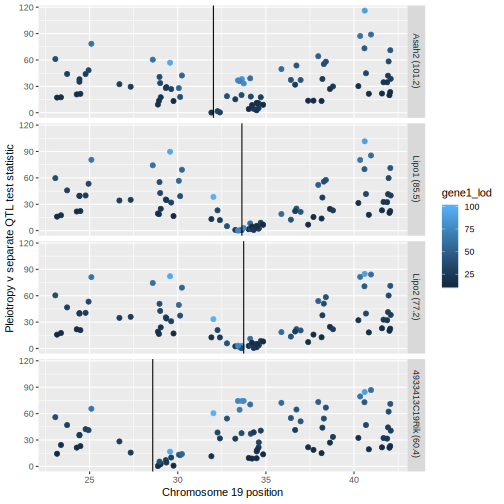
\includegraphics[width = \textwidth]{2018-12-04_lrt-v-middle-of-gene.jpg}
    \caption{Caption}
    \label{fig:middle}
\end{figure}


\subsection{Pleiotropy likelihood ratio test statistics vs. univariate LOD}

\begin{figure}
    \centering
    \includegraphics[width = \textwidth]{2018-12-04_lrt-v-univariate-lod.jpg}
    \caption{Caption}
    \label{fig:lod}
\end{figure}


\subsection{Pleiotropy LRT vs. fitted values correlation}

\begin{figure}
    \centering
    \includegraphics[width = \textwidth]{2018-12-04_lrt-v-corr.jpg}
    \caption{Caption}
    \label{fig:cor}
\end{figure}

\section{Discussion}





\section{References}

\printbibliography


\end{document}
